\documentclass[aspectratio=169]{beamer}

% ── Theme ────────────────────────────────────────────────────────────────────
\usetheme{metropolis}
\usepackage{appendixnumberbeamer}

% ── Packages ─────────────────────────────────────────────────────────────────
\usepackage{amsmath, amssymb}
\usepackage{booktabs}
\usepackage{tikz}
\usetikzlibrary{shapes.geometric, arrows.meta, positioning, fit, calc}
\usepackage{xcolor}
\usepackage{fontawesome5}

% ── Colors ───────────────────────────────────────────────────────────────────
\definecolor{mDark}    {HTML}{23373B}
\definecolor{mMid}     {HTML}{2D6A9F}
\definecolor{mAccent}  {HTML}{E74C3C}
\definecolor{mYellow}  {HTML}{F39C12}
\definecolor{mGreen}   {HTML}{27AE60}
\definecolor{mLight}   {HTML}{ECF0F1}

\setbeamercolor{normal text}       {fg=mDark}
\setbeamercolor{frametitle}        {bg=mDark, fg=white}
\setbeamercolor{title separator}   {fg=mAccent}
\setbeamercolor{progress bar}      {fg=mAccent, bg=mDark!30}
\setbeamercolor{alerted text}      {fg=mAccent}
\setbeamercolor{block title}       {bg=mMid,    fg=white}
\setbeamercolor{block body}        {bg=mMid!10}
\setbeamercolor{block title alerted}{bg=mAccent!85, fg=white}
\setbeamercolor{block body alerted} {bg=mAccent!10}
\setbeamercolor{block title example}{bg=mGreen!75, fg=white}
\setbeamercolor{block body example} {bg=mGreen!10}

% ── Meta ─────────────────────────────────────────────────────────────────────
\title{Interpretability in Deep Learning}
\subtitle{Opening the Black Box}
\author{CAS Trustworthy AI}
\institute{ETH Zürich}
\date{\today}

% ─────────────────────────────────────────────────────────────────────────────
\begin{document}
% ─────────────────────────────────────────────────────────────────────────────

\maketitle

% ── Outline ──────────────────────────────────────────────────────────────────
\begin{frame}{What We Will Cover}
  \setbeamertemplate{section in toc}[sections numbered]
  \tableofcontents
\end{frame}

% =============================================================================
\section{Why Interpretability Matters}
% =============================================================================

\begin{frame}{The Tension at the Heart of Modern AI}
  \begin{columns}[T]
    \begin{column}{0.55\textwidth}
      Deep learning is extraordinarily capable — \alert{and extraordinarily opaque}.

      \vspace{0.8em}
      A radiologist can explain their diagnosis step by step.\\
      A neural network gives you ``cancer: 94\%'' and stops there.

      \vspace{0.8em}
      \textbf{Interpretability} is the field asking:
      \begin{quote}
        \itshape ``What did the model \emph{actually} learn, and why does it make
        the predictions it does?''
      \end{quote}
    \end{column}
    \begin{column}{0.4\textwidth}
      \begin{block}{High-stakes domains}
        \begin{itemize}
          \item[\faHeartbeat] Medical diagnosis
          \item[\faBalanceScale] Legal \& credit decisions
          \item[\faCar] Autonomous driving
          \item[\faShieldAlt] Fraud detection
          \item[\faRobot] LLM-assisted decisions
        \end{itemize}
      \end{block}
    \end{column}
  \end{columns}
\end{frame}

\begin{frame}{The ``Clever Hans'' Lesson}
  \begin{columns}[T]
    \begin{column}{0.55\textwidth}
      In the early 1900s, a horse named \textbf{Clever Hans} appeared to solve
      arithmetic problems. In reality, he was reading \emph{subtle body-language
      cues} from his trainer.

      \vspace{0.7em}
      Neural networks do the same kind of thing:
      \begin{itemize}
        \item A skin-cancer classifier learned to detect \textbf{ruler marks}
              (rulers appear more often next to malignant lesions in training data).
        \item A military tank detector learned to distinguish \textbf{cloudy vs.\ sunny
              days} — tank photos happened to be taken on overcast days.
        \item A COVID X-ray model focused on \textbf{hospital-specific text overlays},
              not lung tissue.
      \end{itemize}
    \end{column}
    \begin{column}{0.4\textwidth}
      \begin{alertblock}{Shortcut Learning}
        Models exploit statistical regularities in training data that are
        \emph{irrelevant to the true task}.
        High test accuracy is \textbf{not} a guarantee of the right reasoning.
      \end{alertblock}

      \vspace{0.6em}
      Interpretability lets us \textbf{audit} these shortcuts before deployment.
    \end{column}
  \end{columns}
\end{frame}

\begin{frame}{Three Motivations for Interpretability}
  \begin{columns}[T]
    \begin{column}{0.32\textwidth}
      \begin{block}{\faWrench\; Debugging}
        Find \emph{why} a model fails on certain inputs.
        Fix data issues, architecture choices, or training artefacts.
      \end{block}
    \end{column}
    \begin{column}{0.32\textwidth}
      \begin{exampleblock}{\faGavel\; Compliance}
        EU GDPR \& AI Act require ``meaningful explanations''
        for automated decisions affecting people.
      \end{exampleblock}
    \end{column}
    \begin{column}{0.32\textwidth}
      \begin{alertblock}{\faUserShield\; Trust}
        Humans adopt AI tools more safely when they understand
        the model's reasoning process.
      \end{alertblock}
    \end{column}
  \end{columns}

  \vspace{1em}
  \begin{center}
    \large \textbf{Interpretability $=$ Debugging $+$ Compliance $+$ Trust}
  \end{center}
\end{frame}

% =============================================================================
\section{A Map of the Field}
% =============================================================================

\begin{frame}{Two Fundamental Distinctions}
  \begin{columns}[T]
    \begin{column}{0.48\textwidth}
      \begin{block}{Intrinsic vs.\ Post-hoc}
        \textbf{Intrinsic:} use a model that is interpretable \emph{by design}
        (decision trees, linear models, rule lists).\\[4pt]
        \textbf{Post-hoc:} take any trained model and apply an explanation method
        on top of it.
      \end{block}
    \end{column}
    \begin{column}{0.48\textwidth}
      \begin{block}{Local vs.\ Global}
        \textbf{Local:} explain \emph{one specific prediction}
        — ``Why did the model say \emph{this} image is a cat?''\\[4pt]
        \textbf{Global:} explain \emph{the model as a whole}
        — ``What patterns did the model learn in general?''
      \end{block}
    \end{column}
  \end{columns}

  \vspace{0.8em}
  Most practical tools are \alert{post-hoc} (they work with any model) and
  cover \alert{both} local and global explanations.
\end{frame}

\begin{frame}{The Interpretability–Accuracy Trade-off}
  \begin{center}
  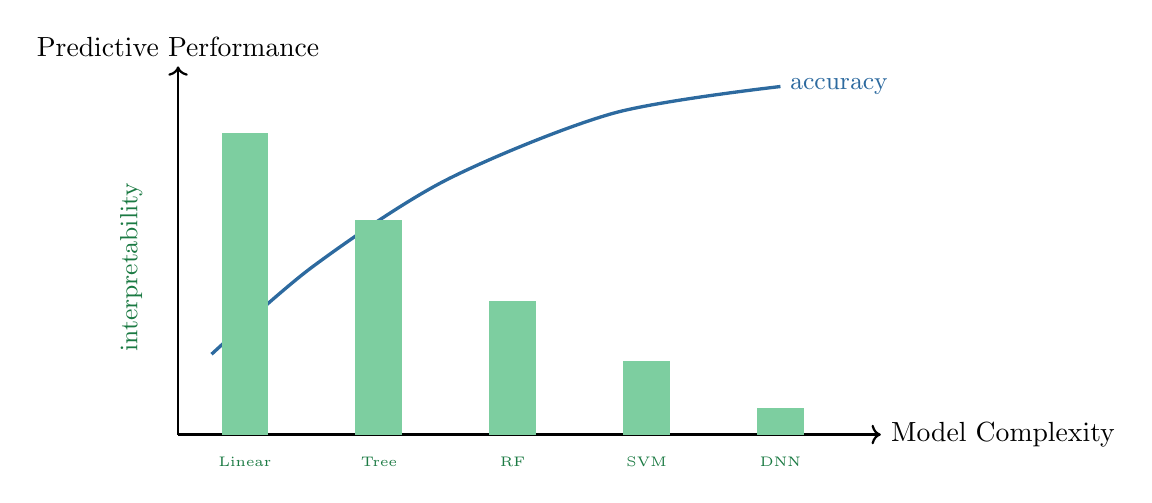
\begin{tikzpicture}[scale=0.85]
    % Axes
    \draw[->, thick] (0,0) -- (10.5,0) node[right] {Model Complexity};
    \draw[->, thick] (0,0) -- (0,5.5)  node[above] {Predictive Performance};

    % Accuracy curve
    \draw[mMid, very thick, bend right=10]
      plot[smooth] coordinates {(0.5,1.2)(2,2.5)(4,3.8)(6.5,4.8)(9,5.2)};
    \node[mMid, right] at (9,5.2) {\small accuracy};

    % Interpretability bar (decreasing)
    \foreach \x/\h in {1/4.5, 3/3.2, 5/2.0, 7/1.1, 9/0.4}{
      \fill[mGreen!60] (\x-0.35,0) rectangle (\x+0.35,\h);
    }
    \node[mGreen!70!black] at (1,-0.4) {\tiny Linear};
    \node[mGreen!70!black] at (3,-0.4) {\tiny Tree};
    \node[mGreen!70!black] at (5,-0.4) {\tiny RF};
    \node[mGreen!70!black] at (7,-0.4) {\tiny SVM};
    \node[mGreen!70!black] at (9,-0.4) {\tiny DNN};

    \node[mGreen!70!black, rotate=90] at (-0.7, 2.5) {\small interpretability};
  \end{tikzpicture}
  \end{center}
  \small Post-hoc methods let us use powerful DNNs \emph{while still gaining insight}
  — at the cost of approximation.
\end{frame}

% =============================================================================
\section{Feature Attribution}
% =============================================================================

\begin{frame}{What Is Feature Attribution?}
  \textbf{Core idea:} assign an importance score to each input feature
  (pixel, word, tabular column) that reflects how much it influenced
  a specific prediction.

  \vspace{0.8em}
  \begin{center}
  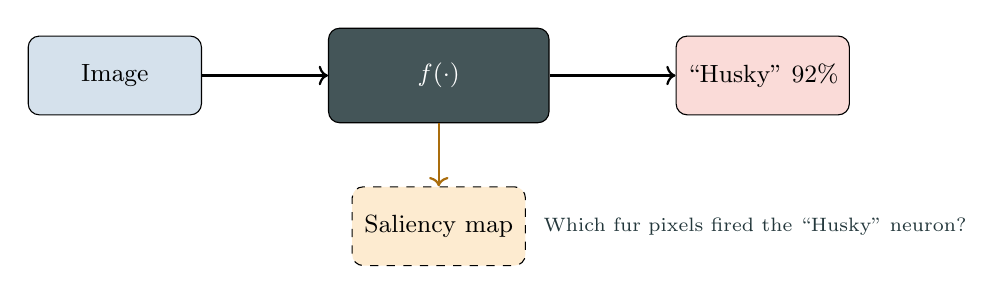
\begin{tikzpicture}[node distance=1.6cm, every node/.style={font=\small}]
    \node[draw, rounded corners, fill=mMid!20, minimum width=2.2cm,
          minimum height=1cm] (img) {Image};
    \node[draw, fill=mDark!85, text=white, minimum width=2.8cm,
          minimum height=1.2cm, right=of img, rounded corners] (f)
          {$f(\cdot)$};
    \node[draw, rounded corners, fill=mAccent!20, minimum width=2.2cm,
          minimum height=1cm, right=of f] (pred) {``Husky'' 92\%};
    \node[draw, dashed, rounded corners, fill=mYellow!20, minimum width=2.2cm,
          minimum height=1cm, below=0.8cm of f] (attr)
          {Saliency map};

    \draw[->, thick] (img) -- (f);
    \draw[->, thick] (f)   -- (pred);
    \draw[->, thick, mYellow!70!black] (f) -- (attr);
    \node[right=0.1cm of attr, font=\scriptsize, text=mDark]
      {Which fur pixels fired the ``Husky'' neuron?};
  \end{tikzpicture}
  \end{center}

  \vspace{0.5em}
  Attribution methods answer this question without retraining the model.
\end{frame}

\begin{frame}{Gradient-Based Attribution}
  \textbf{Intuition:} if a small change in pixel $i$ causes a large change
  in the prediction, that pixel matters.

  \vspace{0.5em}
  \begin{columns}[T]
    \begin{column}{0.52\textwidth}
      \textbf{Vanilla gradients}\\
      Importance $\propto$ how steeply the output rises w.r.t.\ each input.

      \vspace{0.5em}
      \textbf{Problem:} gradients saturate —
      once a feature is ``obviously present'', the gradient is near zero
      even though the feature is critical.

      \vspace{0.7em}
      \textbf{Integrated Gradients} (Sundararajan et al., 2017)\\
      Accumulate gradients along a path from a neutral \emph{baseline}
      (e.g.\ a black image) to the actual input.
      Avoids saturation and satisfies desirable theoretical axioms.
    \end{column}
    \begin{column}{0.44\textwidth}
      \begin{exampleblock}{Analogy}
        Imagine water flowing from a source to a destination.
        Integrated Gradients measures how much each ``channel''
        (feature) carries across the entire path —
        not just at the destination.
      \end{exampleblock}
    \end{column}
  \end{columns}
\end{frame}

\begin{frame}{Grad-CAM: Where Did the Network Look?}
  \textbf{Gradient-weighted Class Activation Mapping} produces a
  \alert{heatmap} on the image showing discriminative regions.

  \vspace{0.6em}
  \begin{columns}[T]
    \begin{column}{0.55\textwidth}
      \textbf{How it works (intuitively):}
      \begin{enumerate}
        \item Pick the last convolutional layer — it retains spatial structure
              while being semantically rich.
        \item Ask: ``How much does each feature map channel contribute to
              the target class score?''
        \item Weight each channel by its importance and blend them into
              one heatmap.
        \item Overlay on the original image.
      \end{enumerate}

      \vspace{0.4em}
      \small No retraining needed. Works for CNNs and,
      with modifications, for transformers (Attention Rollout).
    \end{column}
    \begin{column}{0.4\textwidth}
      \begin{block}{Key insight}
        The gradient tells us \emph{which neurons matter};
        the activation map tells us \emph{where} in the image
        those neurons are responding.
        Combining both gives a spatially-grounded explanation.
      \end{block}
    \end{column}
  \end{columns}
\end{frame}

\begin{frame}{LIME: Locally Faithful Approximations}
  \textbf{Local Interpretable Model-agnostic Explanations} (Ribeiro et al., 2016)

  \vspace{0.5em}
  \begin{columns}[T]
    \begin{column}{0.55\textwidth}
      \textbf{Recipe:}
      \begin{enumerate}
        \item Take the input to be explained.
        \item Create many slightly perturbed versions of it
              (e.g.\ mask out image patches or words).
        \item Query the black-box model on all of them.
        \item Fit a simple, interpretable model (linear regression)
              to mimic the black box \emph{locally}.
        \item The coefficients of the linear model are the explanation.
      \end{enumerate}
    \end{column}
    \begin{column}{0.4\textwidth}
      \begin{alertblock}{Trade-off}
        The linear approximation is only valid
        \emph{near the input of interest}.
        It may be wrong elsewhere — the model is complex globally.
      \end{alertblock}

      \vspace{0.5em}
      \textbf{Model-agnostic:} works for images, text, and tabular data with
      the same algorithm.
    \end{column}
  \end{columns}
\end{frame}

\begin{frame}{SHAP: Principled Feature Attribution}
  \textbf{SHapley Additive exPlanations} (Lundberg \& Lee, 2017) borrows from
  \textbf{cooperative game theory}.

  \vspace{0.5em}
  \begin{columns}[T]
    \begin{column}{0.55\textwidth}
      \textbf{Intuition via a salary analogy:}\\
      A team of players (features) together produce a profit (prediction).
      How much credit does each player deserve?

      \vspace{0.5em}
      Shapley values answer this by averaging each feature's
      contribution over \emph{all possible team combinations}.

      \vspace{0.6em}
      \textbf{Why it is special:}
      \begin{itemize}
        \item Only method satisfying all four fairness axioms simultaneously
        \item Global plots (beeswarm, bar) give dataset-level insight
        \item \texttt{TreeSHAP} is exact and fast for tree ensembles
      \end{itemize}
    \end{column}
    \begin{column}{0.4\textwidth}
      \begin{exampleblock}{Reading a SHAP plot}
        Each row = one feature.\\
        Each dot = one data point.\\
        Position left/right = negative/positive effect.\\
        Color = feature value (red = high, blue = low).
      \end{exampleblock}
    \end{column}
  \end{columns}
\end{frame}

% =============================================================================
\section{Probing \& Concept-Based Methods}
% =============================================================================

\begin{frame}{What Do Individual Neurons Encode?}
  Beyond explaining single predictions, we can ask:
  \textbf{what concepts has the network learned to represent internally?}

  \vspace{0.7em}
  \begin{columns}[T]
    \begin{column}{0.48\textwidth}
      \begin{block}{Network Dissection}
        For each neuron, find the images that maximally activate it.
        Label the concept manually.
        Early layers: edges, colors.
        Middle layers: textures, parts.
        Late layers: whole objects, scenes.
      \end{block}
    \end{column}
    \begin{column}{0.48\textwidth}
      \begin{block}{Probing Classifiers}
        Freeze the network. Train a tiny linear classifier on top
        of layer $\ell$'s representations to predict a concept
        (e.g.\ grammatical person, sentiment, color).\\
        High accuracy $\Rightarrow$ the layer \emph{encodes} that concept.
      \end{block}
    \end{column}
  \end{columns}

  \vspace{0.7em}
  These methods reveal the \alert{representational hierarchy} built by
  gradient descent — often matching human-intuitive stages of processing.
\end{frame}

\begin{frame}{TCAV: Testing with Concept Activation Vectors}
  \textbf{Goal:} does the model rely on a \emph{human-defined concept}
  when making predictions — even if that concept was never in the training labels?

  \vspace{0.6em}
  \begin{columns}[T]
    \begin{column}{0.55\textwidth}
      \textbf{How it works:}
      \begin{enumerate}
        \item Collect a small set of images that \emph{do} and \emph{do not}
              embody the concept (e.g.\ ``striped texture'').
        \item Train a linear classifier in activation space to separate them.
              The decision boundary is the \textbf{concept activation vector} (CAV).
        \item Measure how much moving in the CAV direction increases the
              class score.
      \end{enumerate}
    \end{column}
    \begin{column}{0.4\textwidth}
      \begin{exampleblock}{Famous result}
        A medical classifier was found to heavily rely on the concept
        ``ruler marks'' — a confounder present in dermoscopy datasets,
        not a real signal of malignancy.
      \end{exampleblock}
    \end{column}
  \end{columns}

  \vspace{0.3em}
  \small TCAV requires \emph{no changes} to the model and needs only a handful
  of concept images.
\end{frame}

% =============================================================================
\section{Attention \& Transformers}
% =============================================================================

\begin{frame}{Is Attention Explanation?}
  Transformers compute \textbf{attention weights} between tokens.
  It is tempting to read these as importance scores — ``the model attended to
  \emph{bank} when predicting \emph{money}''.

  \vspace{0.7em}
  \begin{columns}[T]
    \begin{column}{0.48\textwidth}
      \begin{exampleblock}{\faCheck\; Arguments for}
        \begin{itemize}
          \item Directly part of the forward pass
          \item Visualizable and intuitive
          \item Align with human reading patterns in many cases
        \end{itemize}
      \end{exampleblock}
    \end{column}
    \begin{column}{0.48\textwidth}
      \begin{alertblock}{\faTimes\; Arguments against}
        \begin{itemize}
          \item Attention is not attribution (Jain \& Wallace, 2019)
          \item Different attention patterns can produce identical outputs
          \item Multi-head attention is hard to aggregate meaningfully
        \end{itemize}
      \end{alertblock}
    \end{column}
  \end{columns}

  \vspace{0.7em}
  \textbf{Better alternatives:} Attention Rollout, raw attention $\times$ gradient,
  or applying gradient-based attribution inside the transformer.
\end{frame}

% =============================================================================
\section{Mechanistic Interpretability}
% =============================================================================

\begin{frame}{Going Deeper: What Algorithm Is Running?}
  The methods so far tell us \emph{what} a model uses.
  \textbf{Mechanistic interpretability} asks \emph{how} the model computes it —
  reverse-engineering the algorithm implemented by the weights.

  \vspace{0.6em}
  Pioneered by Anthropic, Redwood Research, and others on transformers.

  \vspace{0.5em}
  \begin{block}{Circuits}
    A \textbf{circuit} is a minimal subgraph of the network
    (specific attention heads + MLP neurons + their connections)
    that implements an identifiable computation.
  \end{block}

  \vspace{0.5em}
  \textbf{Example discovered circuits:}
  \begin{itemize}
    \item \textbf{Induction heads} — copy previous patterns,
          enabling in-context learning.
    \item \textbf{Indirect object identification} — in
          ``John gave Mary the ball; she …'', the model resolves the pronoun.
    \item \textbf{Curve detectors} in CNNs — specific neurons that activate on
          curves at particular orientations.
  \end{itemize}
\end{frame}

\begin{frame}{Superposition: Why Neurons Are Hard to Interpret}
  \begin{columns}[T]
    \begin{column}{0.55\textwidth}
      \textbf{Monosemantic neuron:} responds to one concept.
      Easy to interpret.

      \vspace{0.5em}
      \textbf{Polysemantic neuron:} responds to multiple unrelated concepts
      (e.g.\ a neuron in GPT-2 activates for both \emph{cat pictures}
      and \emph{legal text}).

      \vspace{0.5em}
      \textbf{Why?} — The \textbf{superposition hypothesis}:
      \begin{quote}
        \itshape Neural networks represent more features than they have
        neurons by storing them as overlapping directions in activation space.
      \end{quote}

      This makes neuron-level analysis unreliable.
    \end{column}
    \begin{column}{0.4\textwidth}
      \begin{block}{Solution: Sparse Autoencoders (SAEs)}
        Train a sparse autoencoder on the activations.
        It learns to decompose the superimposed directions into
        \emph{monosemantic, human-interpretable features}.

        \vspace{0.3em}
        Recent work (Anthropic, 2024) found millions of interpretable
        features inside Claude, including representations of
        \emph{space, time, and emotion}.
      \end{block}
    \end{column}
  \end{columns}
\end{frame}

% =============================================================================
\section{Evaluation \& Pitfalls}
% =============================================================================

\begin{frame}{How Good Is an Explanation?}
  \textbf{Evaluating explanations is itself an open problem.}

  \vspace{0.5em}
  \begin{columns}[T]
    \begin{column}{0.48\textwidth}
      \textbf{Desired properties:}
      \begin{itemize}
        \item \textbf{Fidelity} — reflects what the model actually does
        \item \textbf{Stability} — similar inputs get similar explanations
        \item \textbf{Sparsity} — concise, not overwhelming
        \item \textbf{Completeness} — attributions account for the full prediction
        \item \textbf{Human-grounded} — useful in practice
      \end{itemize}
    \end{column}
    \begin{column}{0.48\textwidth}
      \begin{alertblock}{The Sanity Check (Adebayo et al., 2018)}
        Randomize the model weights.
        A faithful saliency method \emph{must} produce very different maps.
        Many popular methods (including some gradient methods) failed
        this basic test — their maps look like edge detectors regardless
        of the model.
      \end{alertblock}
    \end{column}
  \end{columns}
\end{frame}

\begin{frame}{Common Pitfalls to Watch Out For}
  \begin{enumerate}
    \setlength\itemsep{0.6em}
    \item \textbf{Plausibility $\neq$ Faithfulness}\\
          An explanation may look convincing to humans but not reflect
          the model's true computation. Humans are easily fooled by
          explanations that confirm their priors.

    \item \textbf{Explanation Gaming}\\
          If explanations become a regulatory checkbox, adversaries can craft
          models that produce ``safe-looking'' explanations
          while still behaving harmfully.
          \emph{Goodhart's Law applies here.}

    \item \textbf{Approximation Artefacts}\\
          LIME and SHAP make assumptions (local linearity, feature
          independence) that may not hold — especially in high dimensions.

    \item \textbf{Scope Mismatch}\\
          A local explanation says nothing about global model behavior.
          Showing one correct heatmap does not mean the model always
          reasons correctly.
  \end{enumerate}
\end{frame}

% =============================================================================
\section{The Bigger Picture}
% =============================================================================

\begin{frame}{Interpretability and AI Safety}
  As AI systems become more capable, interpretability moves from
  \emph{nice-to-have} to \emph{essential}.

  \vspace{0.7em}
  \begin{columns}[T]
    \begin{column}{0.55\textwidth}
      \textbf{Why it matters for safety:}
      \begin{itemize}
        \item Detecting \textbf{deceptive alignment} — a model that behaves well
              during evaluation but has misaligned goals
        \item Auditing for \textbf{dangerous capabilities}
              (e.g.\ knowledge of bioweapons)
        \item Verifying that safety training
              (\textit{RLHF/Constitutional AI}) actually changed
              \emph{internal representations}, not just output style
      \end{itemize}
    \end{column}
    \begin{column}{0.4\textwidth}
      \begin{exampleblock}{Anthropic's bet}
        Mechanistic interpretability is a core part of Anthropic's
        safety research agenda — the idea is that we cannot trust
        a model we cannot read.
      \end{exampleblock}
    \end{column}
  \end{columns}

  \vspace{0.7em}
  \small \textit{``Interpretability is the microscope of AI safety.''} — Neel Nanda
\end{frame}

\begin{frame}{Open Challenges}
  \begin{columns}[T]
    \begin{column}{0.48\textwidth}
      \textbf{Technical:}
      \begin{itemize}
        \item Scaling mechanistic methods to frontier models (GPT-4 scale)
        \item Ground-truth benchmarks for explanation quality
        \item Causal vs.\ correlational explanations
        \item Explaining \emph{emergent} capabilities
      \end{itemize}
    \end{column}
    \begin{column}{0.48\textwidth}
      \textbf{Sociotechnical:}
      \begin{itemize}
        \item Who is the explanation \emph{for}? (regulator, engineer, patient)
        \item Risk of \emph{automation bias} from persuasive explanations
        \item Translating technical explanations into legal accountability
        \item EU AI Act compliance timelines
      \end{itemize}
    \end{column}
  \end{columns}
\end{frame}

% =============================================================================
\section{Summary}
% =============================================================================

\begin{frame}{Key Takeaways}
  \begin{itemize}
    \setlength\itemsep{0.7em}
    \item Deep learning models can learn \textbf{shortcuts} rather than
          the intended task — we need tools to check this.
    \item \textbf{Feature attribution} (SHAP, Grad-CAM, Integrated Gradients)
          tells us what parts of the input drove a prediction.
    \item \textbf{Concept-based methods} (TCAV, probing) reveal what
          \emph{abstractions} the network has built internally.
    \item \textbf{Mechanistic interpretability} is emerging as a powerful
          bottom-up approach — reverse-engineering the model's algorithms.
    \item No single method is universally best. Always apply
          \textbf{sanity checks} and match the explanation to your
          specific use case and audience.
    \item Interpretability is not just academic — it is increasingly a
          \textbf{legal requirement} and a cornerstone of \textbf{AI safety}.
  \end{itemize}
\end{frame}

\begin{frame}{Further Reading}
  \footnotesize
  \begin{itemize}
    \item Ribeiro et al.\ (2016). \textit{``Why Should I Trust You?''} — KDD.
          \hfill \textit{LIME}
    \item Lundberg \& Lee (2017). \textit{A Unified Approach to Interpreting Model Predictions}
          — NeurIPS. \hfill \textit{SHAP}
    \item Selvaraju et al.\ (2017). \textit{Grad-CAM} — ICCV.
    \item Sundararajan et al.\ (2017). \textit{Axiomatic Attribution for Deep Networks}
          — ICML. \hfill \textit{Integrated Gradients}
    \item Kim et al.\ (2018). \textit{Interpretability Beyond Classification with TCAV}
          — ICML.
    \item Adebayo et al.\ (2018). \textit{Sanity Checks for Saliency Maps} — NeurIPS.
    \item Jain \& Wallace (2019). \textit{Attention is not Explanation} — NAACL.
    \item Olah et al.\ (2020). \textit{Zoom In: An Introduction to Circuits}
          — Distill. \hfill \textit{Circuits}
    \item Elhage et al.\ (2022). \textit{Toy Models of Superposition} — Anthropic.
    \item Templeton et al.\ (2024). \textit{Scaling Monosemanticity} — Anthropic.
          \hfill \textit{SAEs}
    \item Molnar (2022). \textit{Interpretable Machine Learning} (free online book).
  \end{itemize}
\end{frame}

\begin{frame}[standout]
  \Huge Thank You
  \vspace{0.8em}
  \normalsize
  Questions \& Discussion
\end{frame}

\end{document}
